\chapter[Introduction]{Introduction}
\markboth{Chap. 1\ \ \enspace Introduction}{Chap 1. Introduction}

\regularsection
\headerregularsection

\updatemylof % to be used with "list of figure divider per chapter" (see PREAMBLE)

\begin{sloppypar} % to suppress overfull box

%Lorem \index{Lorem} ipsum dolor sit amet, consectetuer adipiscing elit \cite{LIUDIMULYO201767}. Ut purus \index{purus} elit,vestibulum ut, placerat ac, adipiscing vitae, felis \citenum{LIUDIMULYO201767}. Curabitur dictum \index{dictum} gravidamauris. Nam arcu libero, nonummy eget, consectetuer id, vulputate a, magna. Donec vehicula augue eu neque \cite{liudimulyo_2018}. Pellentesque habitant morbi tristique senectuset netus et malesuada fames ac turpis egestas \index{egestas}\citenum{liudimulyo_2018}. Mauris ut leo. Cras viverra metusrhoncus sem \cite{2019liudimulyo}. Nulla et lectus vestibulum urna fringilla ultrices. Phasellus eutellus sit amet tortor gravida placerat \citenum{2019liudimulyo}. Integer sapien est, iaculis in, pretium quis,viverra ac, nunc. Praesent eget sem vel leo ultrices bibendum \cite{liudimulyo2020853}. Aenean faucibus. Morbi dolor nulla, malesuada eu, pulvinar at (\ref{fig:figures/paper-iv/fig-1}), mollis ac, nulla. Curabitur auctorsemper nulla \citenum{liudimulyo2020853}. Donec varius orci eget risus. Duis nibh mi, congue eu, accumsaneleifend, sagittis quis, diam. Duis eget orci sit amet orci dignissim rutrum \cite{LIUDIMULYO201767,liudimulyo_2018,2019liudimulyo,liudimulyo2020853,liudimulyo_unpublished1,liudimulyo_unpublished2}.


A vehicle (from Latin: vehiculum \cite{vehicleDef}) is a machine that transports people or cargo. Vehicles include wagons, bicycles, motor vehicles (motorcycles, cars, trucks, buses), railed vehicles (trains, trams), watercraft (ships, boats), amphibious vehicles (screw-propelled vehicle, hovercraft), aircraft (airplanes, helicopters, aerostat) and spacecraft \cite{wikipediaVehicle}. Land vehicles are classified broadly by what is used to apply steering and drive forces against the ground: wheeled, tracked, railed or skied. ISO 3833-1977 is the standard, also internationally used in legislation, for road vehicles types, terms and definitions. Vehicle detection and vehicle type recognition is a practical application of machine learning concepts and is directly applicable for various operations in a traffic surveillance system contributing to an intelligent traffic surveillance system. We will introduce the processing of automatic vehicle detection and recognition using static image datasets. Further using the same technique, we shall improvise vehicle detection by using live CCTV surveillance. The surveillance system includes detection of moving vehicles and recognizing them, counting number of vehicles and verification of their permit with the organization \cite{SriashikaAddala2020}.

Intelligent vehicle detection and counting are becoming increasingly important in the field of highway management. However, due to the different sizes of vehicles, their detection remains a challenge that directly affects the accuracy of vehicle counts. To address this issue, this paper proposes a vision-based vehicle detection and counting system. In the proposed vehicle detection and counting system, the highway road surface in the image is first extracted and divided into a remote area; the method is crucial for improving vehicle detection. Then, the vehicle trajectories are obtained by the ORB algorithm. Finally, the above two areas are placed into the YOLOv5 network to detect the type and location of the vehicle. Several highway surveillance videos based on different scenes are used to verify the proposed methods. The experimental results verify that using the proposed segmentation method can provide higher detection accuracy, especially for the detection of small vehicle object \cite{SongH2019}. 

Vehicle detection and statistics in highway monitoring video scenes are of considerable significance to intelligent traffic management and control of the highway. With the popular installation of traffic surveillance cameras, a vast database of traffic video footage has been obtained for analysis. Generally, at a high viewing angle, a more-distant road surface can be considered. The object size of the vehicle changes greatly at this viewing angle, and the detection accuracy of a small object far away from the road is low. In the face of complex camera scenes, it is essential to effectively solve the above problems and further apply them \cite{SongH2019}. 

A CCTV camera is a very essential part of an intelligent traffic surveillance framework . It is simply the automated process of monitoring the traffic in a particular area and detecting vehicles for further action, as shown in the diagram. The captured images can provide valuable clues to the cops and other public essential tracking services, such as vehicle’s license plate number, time and motion of vehicle, details associated with the driver, etc.. which all may lead to evidence of some crime or any unforeseen or unfortunate incidents . Earlier people used to process images manually. In fact, this system is still going on in India, whereas countries like the USA also have implemented automated machines- CCTVs that function 24x7 and take immediate action via signaling too. Manual work has always been proven slower and less efficient due to human errors and many other factors that affect living beings. Keeping these points in mind and moving with the advancement of technologies, many innovative thinkers have developed certain intelligent traffic control systems using various techniques. This research is based upon the combination of two prior-made researches by scholars whose works have been published \cite{Baran2016}.

\end{sloppypar}

\begin{figure} % \begin{figure} will let LaTeX decide the best figure placement for you ; \begin{figure}[H] for forcing the figure placement here ; in the bottom, \begin{figure}[!b] ; top of the page, \begin{figure}[!t]
    \centering
    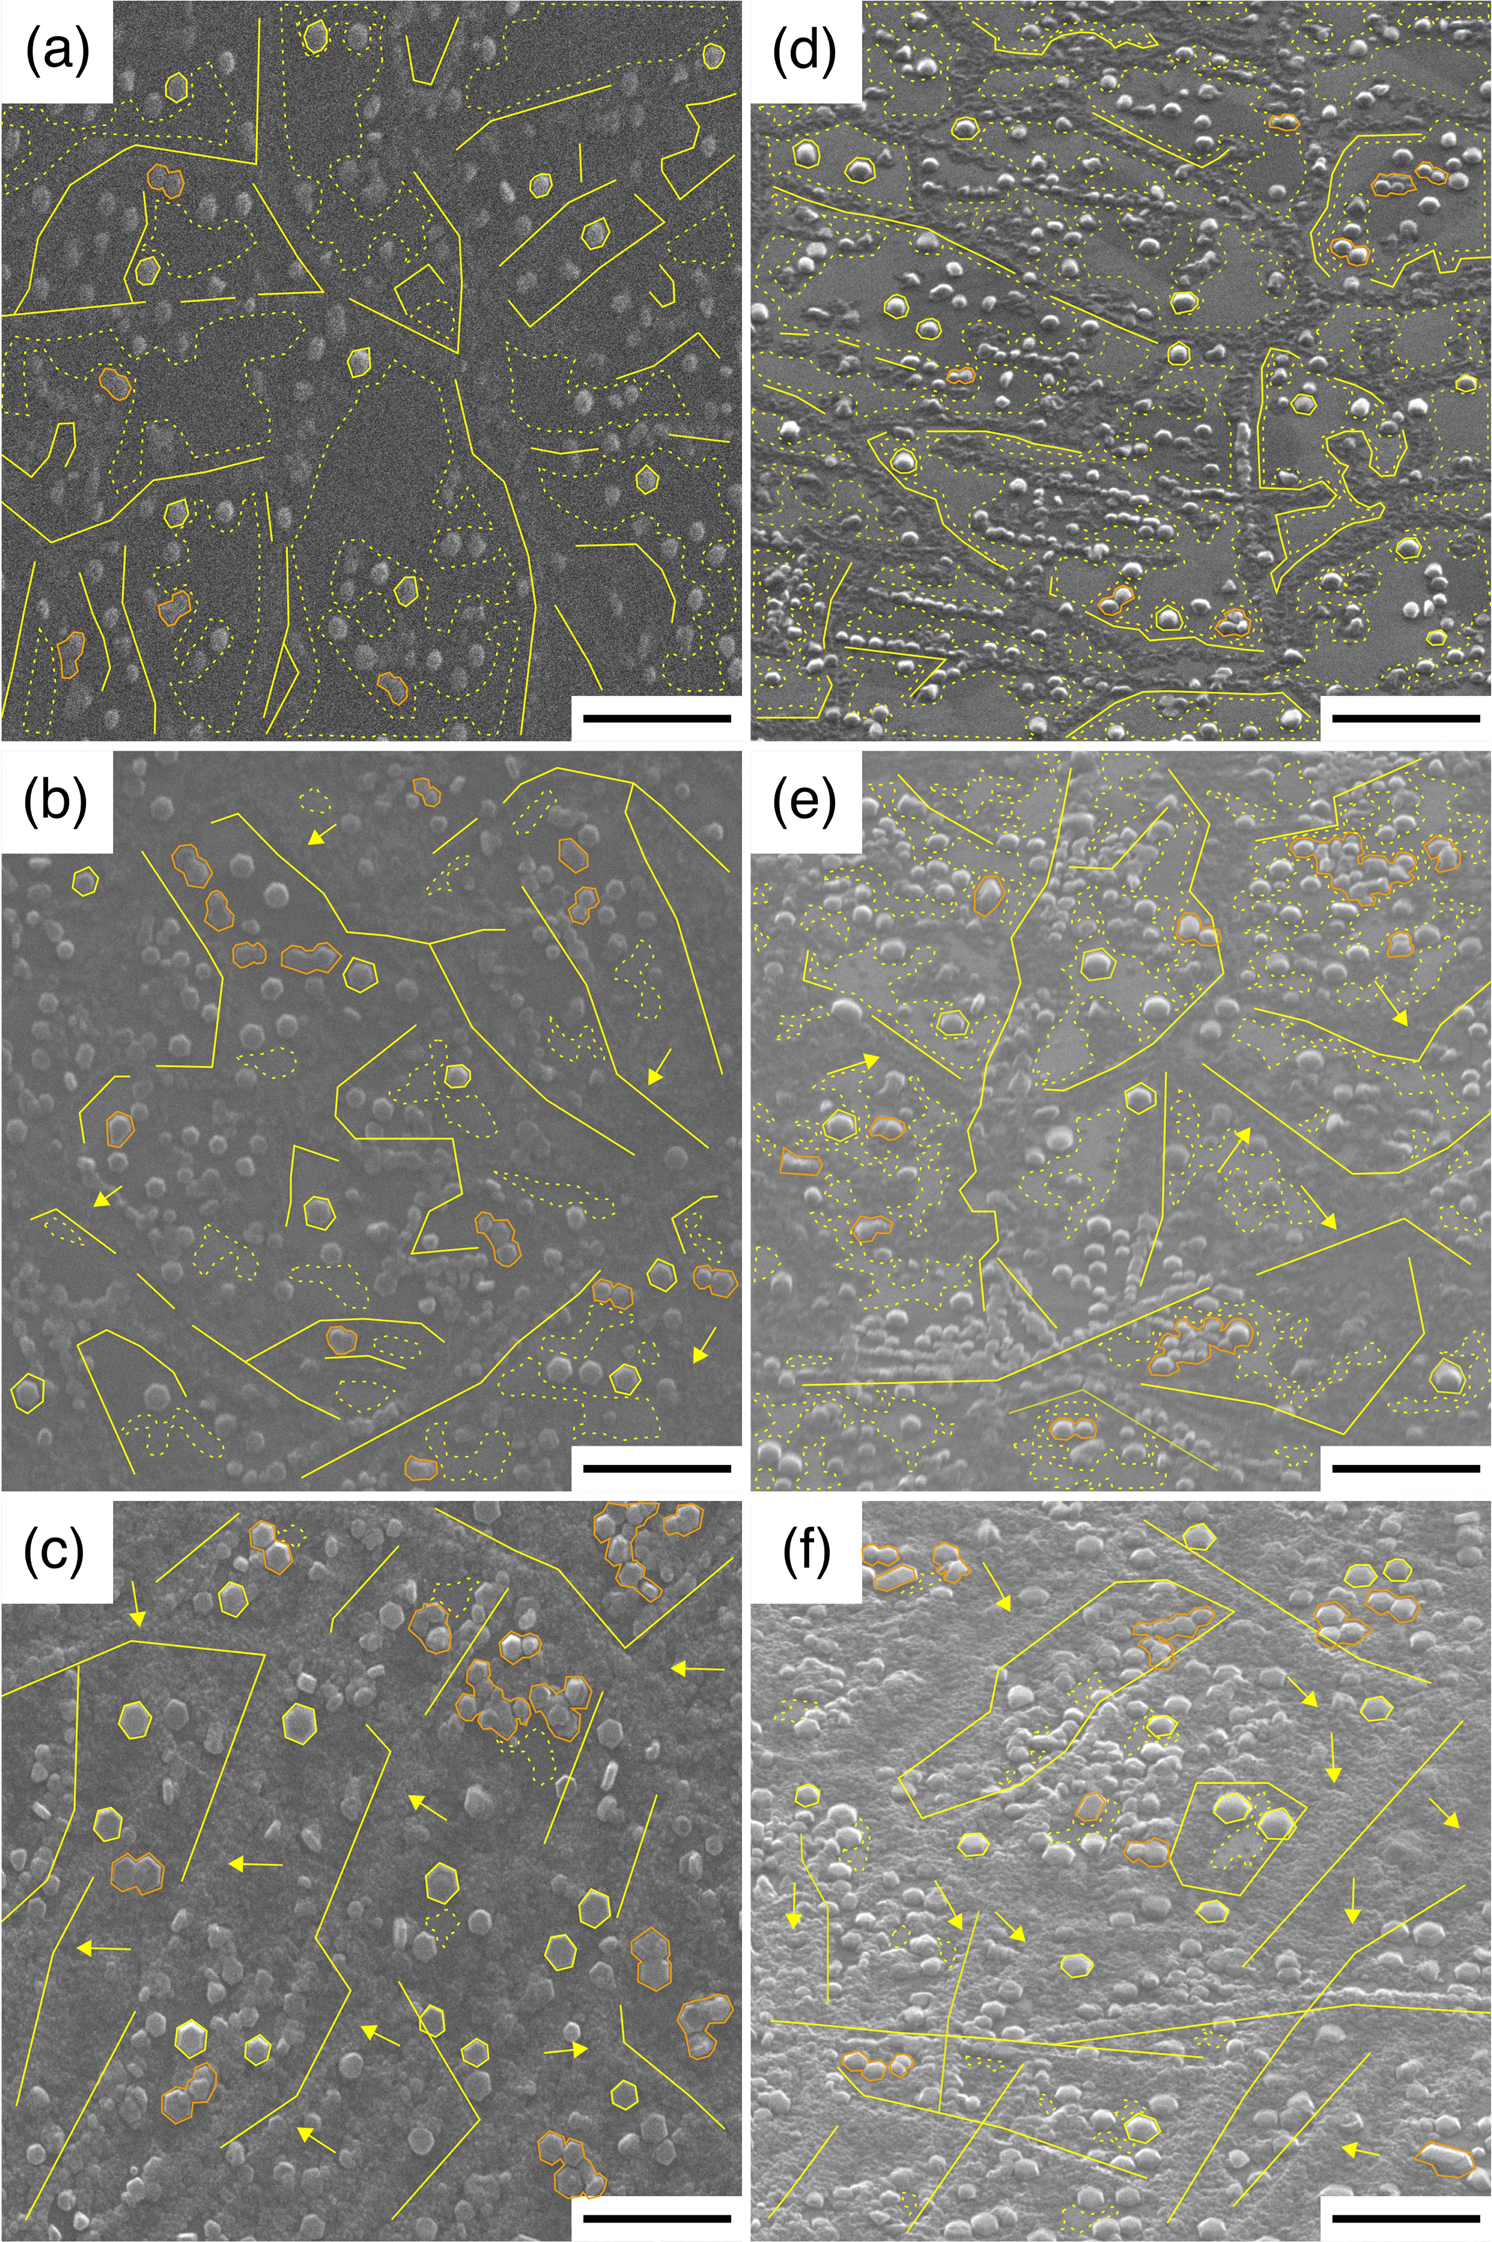
\includegraphics[width=0.95\textwidth]{figures/paper-iv/fig-1.png}
    \caption[SEM images of AlN on graphene formed via different MEE cycles]{SEM images of AlN on graphene formed via different MEE cycles. (\textbf{a},\textbf{d}), (\textbf{b},\textbf{e}) and (\textbf{c},\textbf{f}) are (top-, bird’s eye-view) SEM images of samples A1, A2 and A3, respectively. Scale bars are 1 {\textmu}m. Features marked with yellow lines, yellow (orange) contours and yellow dashed outlines are high-density AlN nanostructures grown along line defects of graphene, individual (coalesced) AlN islands and areas of exposed graphene, respectively. Yellow arrows in samples A2 and A3 show the lateral growth of AlN nanostructures that initially nucleate at the line defects of graphene in sample A1 (adapted with permission from ref. \citenum{liudimulyo2020853} \copyright \ Liudi Mulyo \textit{et al}, 2020.}
    \label{fig:figures/paper-iv/fig-1}
\end{figure}

\section{Section 1 in chapter 1}
\lipsum[2]

\begin{equation}
    EQE = \frac{q \times P_{opt}}{I \times h\nu}
\end{equation}

\lipsum[3-4]

\subsection{Subsection 1.1 of section 1 in chapter 1}
\lipsum[5-7]

\subsection{Subsection 1.2 of section 1 in chapter 1}
\lipsum[8-10]

\clearpage\phantomsection % to fix wrong hyperref to this section
\section[Long section title displayed in the table of content]{Short section title in the chapter}
\sectionmark{Even shorter title on the header}
\lipsum[11-20]

\subsection{Subsection 1.2 of section 2 in chapter 1}
\lipsum[13-14]

%=======================================================================
%%% References 

% \clearpage
\phantomsection
\specialsection % put an indent, see preamble
\headerspecialsection

{\hypersetup{urlcolor=ntnu,linkcolor=sophia} % set clickable URL title color to black, not ntnu like in the main document

\bibliographystyle{unsrtnat-mod}  % NATBIB ref style
\bibliography{references}
}
